\section{Introduction}
\label{sec:intro}

Modern end-to-end driving stacks are multi-modal by construction: given a scene, the planner proposes $K$ candidate trajectories, and the vehicle executes one of them.
The field's dominant reporting convention, minADE@$K$ and its closed-loop analogues, scores the \emph{best} of the $K$ candidates---implicitly assuming an oracle selector that deployment does not have.
What the vehicle actually achieves is set by the candidate it \emph{selects}; the difference between the oracle's outcome and the selected outcome is the \emph{selected regret}, and it is the quantity this paper measures, models, and reduces.
Under a strong 10B-parameter driving VLA generator with $K{=}8$ sampled candidates, we find the selected regret of a trained geometry-only selector is \AbsLegacyKEightRegret{} official-score points per scene (scale $[0,1]$), against an oracle gap of zero---small in absolute terms, but persistent, and invisible to minADE-style reporting.

One route to closing this gap is \emph{explicit imagination}.
WoTE~\cite{li2025wote} trains a BEV world model alongside the planner, autoregressively imagines each candidate's future BEV state, and scores the imagined futures with imitation and simulation-based submetric rewards.
This buys online evaluation at the cost of a purpose-trained world model, per-candidate rollout compute at inference time, and supervision plumbed from simulator submetrics.

This paper asks the opposite question: \emph{does the generator's own forward pass already contain the scene knowledge a selector needs?}
The intuition is that a driving VLA trained to produce good trajectories must internally represent where hazards are, which maneuvers are viable, and how the scene constrains them---an \emph{amortized} form of the same consequence knowledge a world model would compute online.
If that knowledge is readable from activations the planner computes anyway, online evaluation becomes representation \emph{reuse}: zero VLA training, zero inference-time rollouts, and a selector head small enough to be free at deployment.

Concretely, we capture the final-layer hidden states of the frozen VLA's prompt prefill \emph{during the same forward pass that generates the candidates}---the candidates and the representation are provably co-produced (the pooled scene vector is bit-exactly the last row of the captured sequence, hash-verified at capture time; \cref{sec:capture}).
A \EffParams-parameter decomposed value head (\cref{sec:head}) reads this representation and scores each candidate independently in \EffLtMedianMs~ms for all $K{=}8$, with \EffLtMemMb~MB peak incremental memory.

Three findings structure our results.
\textbf{First}, the frozen representation carries a real, scene-specific, causally verified selection signal: on \nScenes{} prospectively frozen, never-before-touched scenes, the representation-informed head beats a parameter-matched scene-blind control on selected regret (\MThreeKEightRegretCI) and tie-aware top-1 agreement (\MThreeKEightTopOneCI), while wrong-scene substitution and representation zeroing degrade selection (\cref{sec:res-signal}).
\textbf{Second}, and counterintuitively, \emph{more context hurts}: a matched-capacity reader given the full $3{,}086\times4{,}096$ prefill sequence is CI-supported \emph{worse} than the same architecture reading only the last token (regret \MOneKEightRegretCI, top-1 \MOneKEightTopOneCI; \cref{sec:res-onetoken}).
The generator has already summarized the scene into its terminal prefill state; re-reading its full working memory dilutes the signal under a fixed parameter budget.
\textbf{Third}, effects of this size demand statistical care the area rarely applies.
Every confirmatory study in this paper was preregistered with frozen decision gates before outcomes existed; endpoints use paired scene bootstrap confidence intervals; cohorts advance on a ladder from development scenes to prospectively frozen untouched scenes to a sealed confirmation set that is never opened until a winner is frozen; and every number in this paper is machine-read from hash-locked result records (\cref{sec:program}).
\iffnonedone\else
The program culminates in a comparison against the trained geometry incumbent that is \emph{adequately powered by design}: the sample size ($N=\FnNTotal$ scenes) was derived from the locked pilot effect (MDE $\FnMde$, paired SD $\FnSdPaired$) to reach $1-\beta=\FnPowerAchieved$ at two-sided $\alpha=0.05$.
\fi

Our contributions are:
\begin{itemize}
  \item \textbf{C1 --- Same-prefill capture and an open evaluation program.} A capture protocol that provably ties the reused representation to the exact forward pass that produced the candidates, embedded in an evaluation design (preregistration, frozen gates, cohort ladder, causal ablations, sealed confirmation) that we argue should become standard for selector claims (\cref{sec:capture,sec:program}).
  \item \textbf{C2 --- Positive result.} The frozen VLA's last prefill token supports scene-specific trajectory selection with CI-supported gains on both primary endpoints, replicated prospectively on untouched scenes and causally verified by ablation (\cref{sec:res-signal}).
  \item \textbf{C3 --- Negative result.} Under matched capacity, the full prefill sequence is CI-supported worse than its last token alone---a ``more context hurts'' finding with direct architectural consequences for representation-reuse selectors (\cref{sec:res-onetoken}).
  \item \textbf{C4 --- Powered incumbent verdict.}
  \iffnonedone
    \iffnonepass
      At $1-\beta=0.80$ power, the representation-based selector surpasses the tuned trajectory-geometry incumbent on the promoting endpoint with preregistered non-inferiority on the others (\cref{sec:res-incumbent}).
    \else
      At $1-\beta=0.80$ power, the representation-based selector does \emph{not} displace the tuned trajectory-geometry incumbent; we report this as a clean, adequately powered boundary on when representation reuse pays, together with the conditions under which the representation \emph{does} add value (\cref{sec:res-incumbent}).
    \fi
  \else
    An adequately powered ($N=\FnNTotal$, $1-\beta=0.80$), preregistered verdict on whether the reused representation displaces a tuned trajectory-geometry incumbent (\cref{sec:res-incumbent}). \todo{FN1 lands $\sim$Aug 10; both outcome branches are pre-written.}
  \fi
\end{itemize}

\begin{figure}[t]
  \centering
  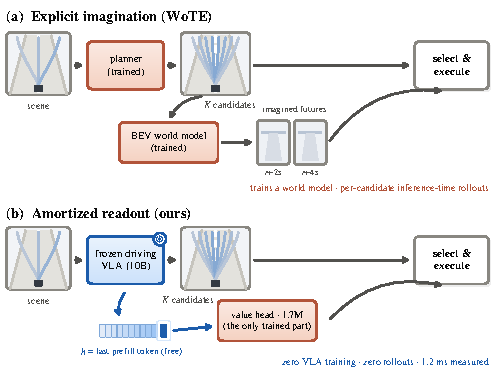
\includegraphics[width=\linewidth]{figs/fig1_teaser.pdf}
  \caption{\textbf{Two routes to online trajectory evaluation.}
  \emph{Top (explicit imagination, WoTE~\cite{li2025wote}):} a purpose-trained BEV world model autoregressively rolls out each candidate's future, then scores the imagined states.
  \emph{Bottom (ours, amortized):} the frozen driving VLA's own prompt prefill---computed anyway to generate the candidates---already summarizes the scene; its last hidden token feeds a \EffParams-parameter value head that scores all $K{=}8$ candidates in \EffLtMedianMs\,ms with zero inference-time rollouts and zero VLA training.}
  \label{fig:teaser}
\end{figure}
